\documentclass[1p]{elsarticle_modified}
%\bibliographystyle{elsarticle-num}

%\usepackage[colorlinks]{hyperref}
%\usepackage{abbrmath_seonhwa} %\Abb, \Ascr, \Acal ,\Abf, \Afrak
\usepackage{amsfonts}
\usepackage{amssymb}
\usepackage{amsmath}
\usepackage{amsthm}
\usepackage{scalefnt}
\usepackage{amsbsy}
\usepackage{kotex}
\usepackage{caption}
\usepackage{subfig}
\usepackage{color}
\usepackage{graphicx}
\usepackage{xcolor} %% white, black, red, green, blue, cyan, magenta, yellow
\usepackage{float}
\usepackage{setspace}
\usepackage{hyperref}

\usepackage{tikz}
\usetikzlibrary{arrows}

\usepackage{multirow}
\usepackage{array} % fixed length table
\usepackage{hhline}

%%%%%%%%%%%%%%%%%%%%%
\makeatletter
\renewcommand*\env@matrix[1][\arraystretch]{%
	\edef\arraystretch{#1}%
	\hskip -\arraycolsep
	\let\@ifnextchar\new@ifnextchar
	\array{*\c@MaxMatrixCols c}}
\makeatother %https://tex.stackexchange.com/questions/14071/how-can-i-increase-the-line-spacing-in-a-matrix
%%%%%%%%%%%%%%%

\usepackage[normalem]{ulem}

\newcommand{\msout}[1]{\ifmmode\text{\sout{\ensuremath{#1}}}\else\sout{#1}\fi}
%SOURCE: \msout is \stkout macro in https://tex.stackexchange.com/questions/20609/strikeout-in-math-mode

\newcommand{\cancel}[1]{
	\ifmmode
	{\color{red}\msout{#1}}
	\else
	{\color{red}\sout{#1}}
	\fi
}

\newcommand{\add}[1]{
	{\color{blue}\uwave{#1}}
}

\newcommand{\replace}[2]{
	\ifmmode
	{\color{red}\msout{#1}}{\color{blue}\uwave{#2}}
	\else
	{\color{red}\sout{#1}}{\color{blue}\uwave{#2}}
	\fi
}

\newcommand{\Sol}{\mathcal{S}} %segment
\newcommand{\D}{D} %diagram
\newcommand{\A}{\mathcal{A}} %arc


%%%%%%%%%%%%%%%%%%%%%%%%%%%%%5 test

\def\sl{\operatorname{\textup{SL}}(2,\Cbb)}
\def\psl{\operatorname{\textup{PSL}}(2,\Cbb)}
\def\quan{\mkern 1mu \triangleright \mkern 1mu}

\theoremstyle{definition}
\newtheorem{thm}{Theorem}[section]
\newtheorem{prop}[thm]{Proposition}
\newtheorem{lem}[thm]{Lemma}
\newtheorem{ques}[thm]{Question}
\newtheorem{cor}[thm]{Corollary}
\newtheorem{defn}[thm]{Definition}
\newtheorem{exam}[thm]{Example}
\newtheorem{rmk}[thm]{Remark}
\newtheorem{alg}[thm]{Algorithm}

\newcommand{\I}{\sqrt{-1}}
\begin{document}

%\begin{frontmatter}
%
%\title{Boundary parabolic representations of knots up to 8 crossings}
%
%%% Group authors per affiliation:
%\author{Yunhi Cho} 
%\address{Department of Mathematics, University of Seoul, Seoul, Korea}
%\ead{yhcho@uos.ac.kr}
%
%
%\author{Seonhwa Kim} %\fnref{s_kim}}
%\address{Center for Geometry and Physics, Institute for Basic Science, Pohang, 37673, Korea}
%\ead{ryeona17@ibs.re.kr}
%
%\author{Hyuk Kim}
%\address{Department of Mathematical Sciences, Seoul National University, Seoul 08826, Korea}
%\ead{hyukkim@snu.ac.kr}
%
%\author{Seokbeom Yoon}
%\address{Department of Mathematical Sciences, Seoul National University, Seoul, 08826,  Korea}
%\ead{sbyoon15@snu.ac.kr}
%
%\begin{abstract}
%We find all boundary parabolic representation of knots up to 8 crossings.
%
%\end{abstract}
%\begin{keyword}
%    \MSC[2010] 57M25 
%\end{keyword}
%
%\end{frontmatter}

%\linenumbers
%\tableofcontents
%
\newcommand\colored[1]{\textcolor{white}{\rule[-0.35ex]{0.8em}{1.4ex}}\kern-0.8em\color{red} #1}%
%\newcommand\colored[1]{\textcolor{white}{ #1}\kern-2.17ex	\textcolor{white}{ #1}\kern-1.81ex	\textcolor{white}{ #1}\kern-2.15ex\color{red}#1	}

{\Large $\underline{11a_{54}~(K11a_{54})}$}

\setlength{\tabcolsep}{10pt}
\renewcommand{\arraystretch}{1.6}
\vspace{1cm}\begin{tabular}{m{100pt}>{\centering\arraybackslash}m{274pt}}
\multirow{5}{120pt}{
	\centering
	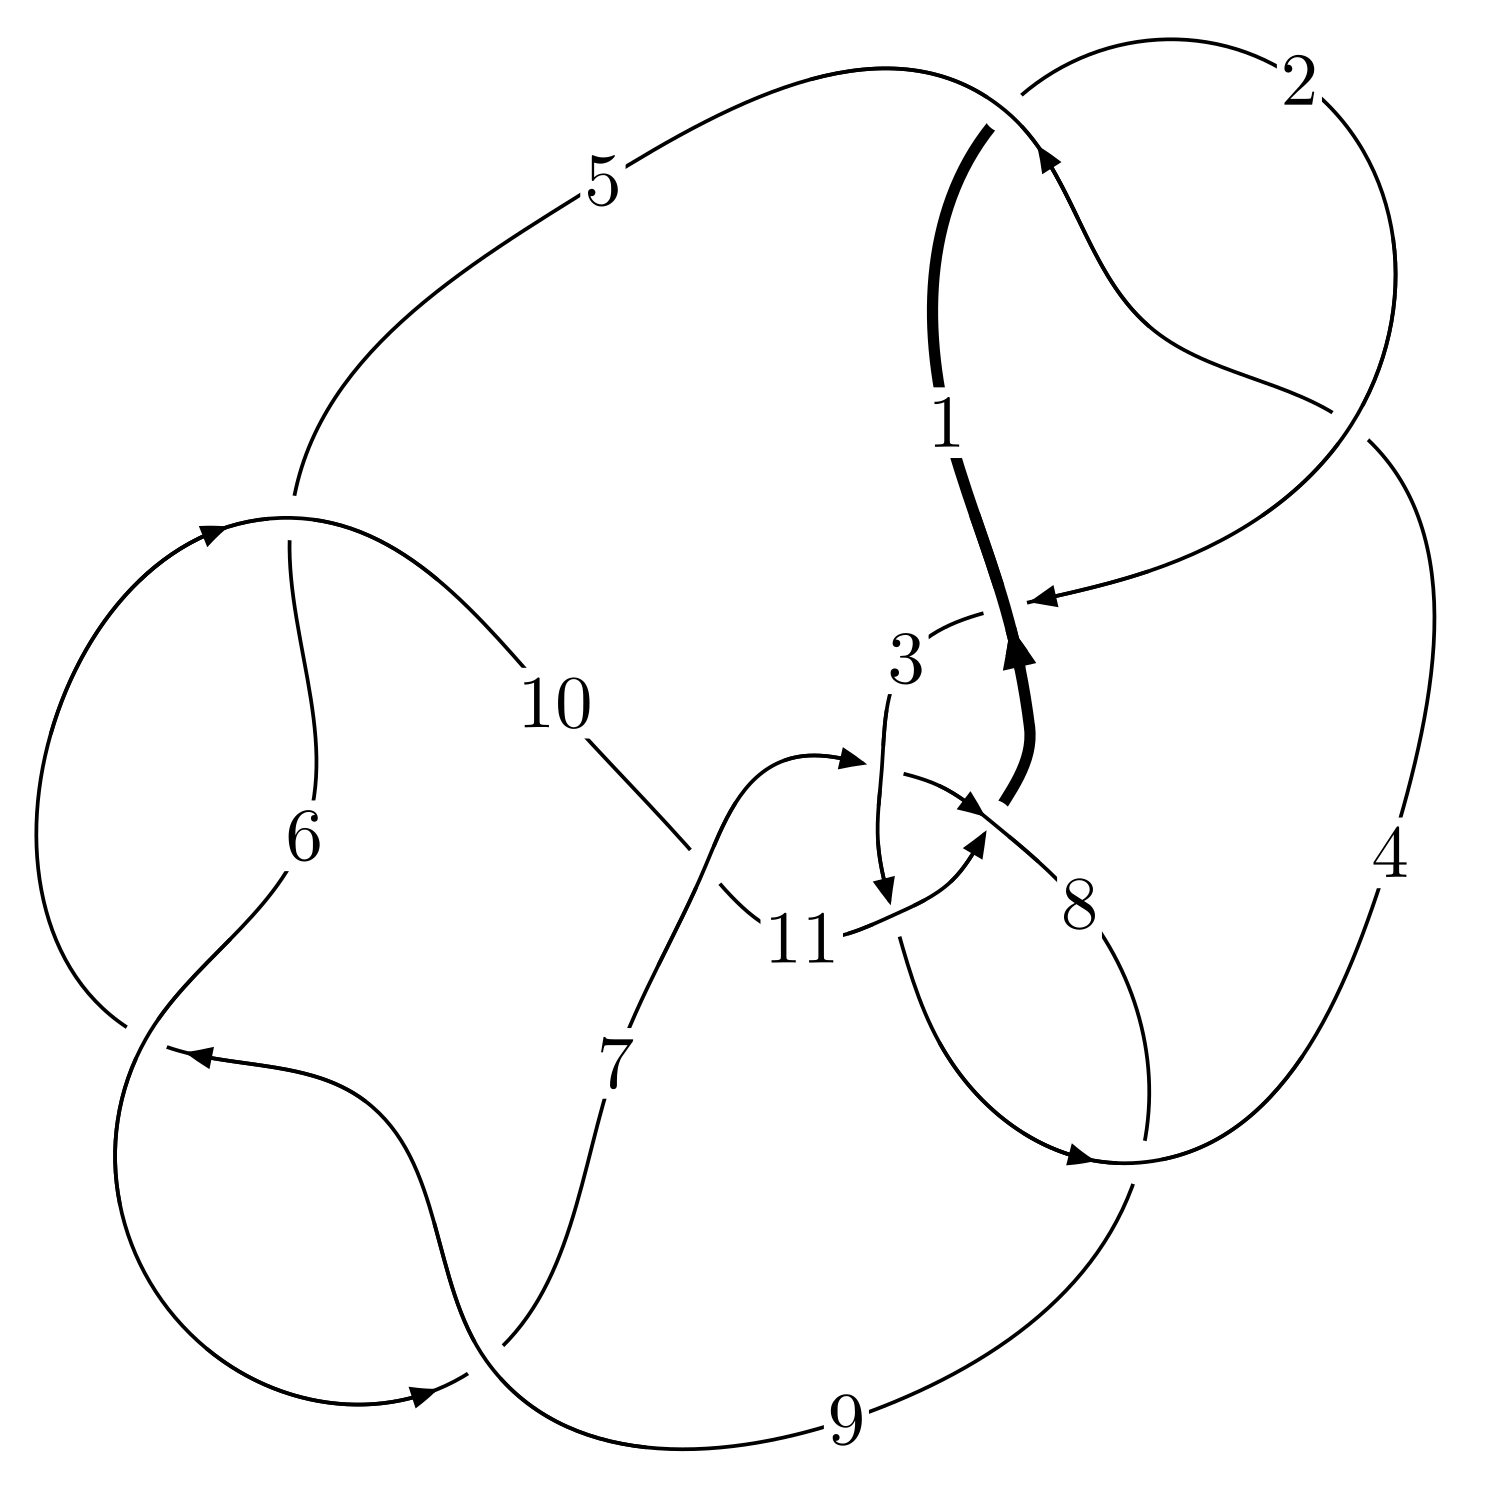
\includegraphics[width=112pt]{../../../GIT/diagram.site/Diagrams/png/303_11a_54.png}\\
\ \ \ A knot diagram\footnotemark}&
\allowdisplaybreaks
\textbf{Linearized knot diagam} \\
\cline{2-2}
 &
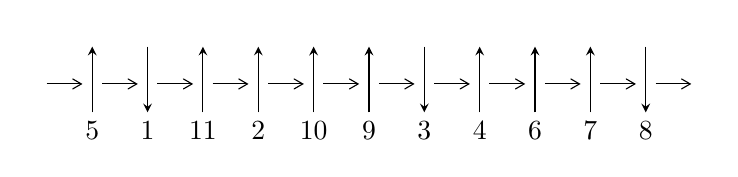
\begin{tikzpicture}[x=20pt, y=17pt]
	% nodes
	\node (C0) at (0, 0) {};
	\node (C1) at (1, 0) {};
	\node (C1U) at (1, +1) {};
	\node (C1D) at (1, -1) {5};

	\node (C2) at (2, 0) {};
	\node (C2U) at (2, +1) {};
	\node (C2D) at (2, -1) {1};

	\node (C3) at (3, 0) {};
	\node (C3U) at (3, +1) {};
	\node (C3D) at (3, -1) {11};

	\node (C4) at (4, 0) {};
	\node (C4U) at (4, +1) {};
	\node (C4D) at (4, -1) {2};

	\node (C5) at (5, 0) {};
	\node (C5U) at (5, +1) {};
	\node (C5D) at (5, -1) {10};

	\node (C6) at (6, 0) {};
	\node (C6U) at (6, +1) {};
	\node (C6D) at (6, -1) {9};

	\node (C7) at (7, 0) {};
	\node (C7U) at (7, +1) {};
	\node (C7D) at (7, -1) {3};

	\node (C8) at (8, 0) {};
	\node (C8U) at (8, +1) {};
	\node (C8D) at (8, -1) {4};

	\node (C9) at (9, 0) {};
	\node (C9U) at (9, +1) {};
	\node (C9D) at (9, -1) {6};

	\node (C10) at (10, 0) {};
	\node (C10U) at (10, +1) {};
	\node (C10D) at (10, -1) {7};

	\node (C11) at (11, 0) {};
	\node (C11U) at (11, +1) {};
	\node (C11D) at (11, -1) {8};
	\node (C12) at (12, 0) {};

	% arrows
	\draw[->,>={angle 60}]
	(C0) edge (C1) (C1) edge (C2) (C2) edge (C3) (C3) edge (C4) (C4) edge (C5) (C5) edge (C6) (C6) edge (C7) (C7) edge (C8) (C8) edge (C9) (C9) edge (C10) (C10) edge (C11) (C11) edge (C12) ;	\draw[->,>=stealth]
	(C1D) edge (C1U) (C2U) edge (C2D) (C3D) edge (C3U) (C4D) edge (C4U) (C5D) edge (C5U) (C6D) edge (C6U) (C7U) edge (C7D) (C8D) edge (C8U) (C9D) edge (C9U) (C10D) edge (C10U) (C11U) edge (C11D) ;
	\end{tikzpicture} \\
\hhline{~~} \\& 
\textbf{Solving Sequence} \\ \cline{2-2} 
 &
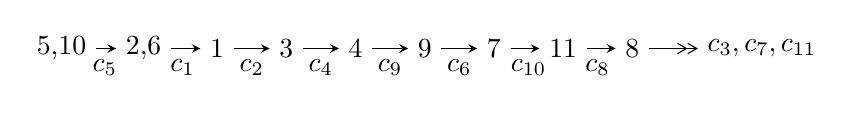
\begin{tikzpicture}[x=25pt, y=7pt]
	% node
	\node (A0) at (-1/8, 0) {5,10};
	\node (A1) at (17/16, 0) {2,6};
	\node (A2) at (17/8, 0) {1};
	\node (A3) at (25/8, 0) {3};
	\node (A4) at (33/8, 0) {4};
	\node (A5) at (41/8, 0) {9};
	\node (A6) at (49/8, 0) {7};
	\node (A7) at (57/8, 0) {11};
	\node (A8) at (65/8, 0) {8};
	\node (C1) at (1/2, -1) {$c_{5}$};
	\node (C2) at (13/8, -1) {$c_{1}$};
	\node (C3) at (21/8, -1) {$c_{2}$};
	\node (C4) at (29/8, -1) {$c_{4}$};
	\node (C5) at (37/8, -1) {$c_{9}$};
	\node (C6) at (45/8, -1) {$c_{6}$};
	\node (C7) at (53/8, -1) {$c_{10}$};
	\node (C8) at (61/8, -1) {$c_{8}$};
	\node (A9) at (10, 0) {$c_{3},c_{7},c_{11}$};

	% edge
	\draw[->,>=stealth]	
	(A0) edge (A1) (A1) edge (A2) (A2) edge (A3) (A3) edge (A4) (A4) edge (A5) (A5) edge (A6) (A6) edge (A7) (A7) edge (A8) ;
	\draw[->>,>={angle 60}]	
	(A8) edge (A9);
\end{tikzpicture} \\ 

\end{tabular} \\

\footnotetext{
The image of knot diagram is generated by the software ``\textbf{Draw programme}" developed by Andrew Bartholomew(\url{http://www.layer8.co.uk/maths/draw/index.htm\#Running-draw}), where we modified some parts for our purpose(\url{https://github.com/CATsTAILs/LinksPainter}).
}\phantom \\ \newline 
\centering \textbf{Ideals for irreducible components\footnotemark of $X_{\text{par}}$} 
 
\begin{align*}
I^u_{1}&=\langle 
-2.90257\times10^{44} u^{68}+2.07176\times10^{44} u^{67}+\cdots+1.04013\times10^{45} b-2.13904\times10^{44},\\
\phantom{I^u_{1}}&\phantom{= \langle  }-5.37164\times10^{44} u^{68}+1.14801\times10^{45} u^{67}+\cdots+1.04013\times10^{45} a-2.55357\times10^{45},\;u^{69}- u^{68}+\cdots+5 u+1\rangle \\
\\
\end{align*}
\raggedright * 1 irreducible components of $\dim_{\mathbb{C}}=0$, with total 69 representations.\\
\footnotetext{All coefficients of polynomials are rational numbers. But the coefficients are sometimes approximated in decimal forms when there is not enough margin.}
\newpage
\renewcommand{\arraystretch}{1}
\centering \section*{I. $I^u_{1}= \langle -2.90\times10^{44} u^{68}+2.07\times10^{44} u^{67}+\cdots+1.04\times10^{45} b-2.14\times10^{44},\;-5.37\times10^{44} u^{68}+1.15\times10^{45} u^{67}+\cdots+1.04\times10^{45} a-2.55\times10^{45},\;u^{69}- u^{68}+\cdots+5 u+1 \rangle$}
\flushleft \textbf{(i) Arc colorings}\\
\begin{tabular}{m{7pt} m{180pt} m{7pt} m{180pt} }
\flushright $a_{5}=$&$\begin{pmatrix}1\\0\end{pmatrix}$ \\
\flushright $a_{10}=$&$\begin{pmatrix}0\\u\end{pmatrix}$ \\
\flushright $a_{2}=$&$\begin{pmatrix}0.516440 u^{68}-1.10372 u^{67}+\cdots-0.812598 u+2.45506\\0.279059 u^{68}-0.199183 u^{67}+\cdots-2.53271 u+0.205651\end{pmatrix}$ \\
\flushright $a_{6}=$&$\begin{pmatrix}1\\- u^2\end{pmatrix}$ \\
\flushright $a_{1}=$&$\begin{pmatrix}0.237382 u^{68}-0.904533 u^{67}+\cdots+1.72012 u+2.24940\\0.279059 u^{68}-0.199183 u^{67}+\cdots-2.53271 u+0.205651\end{pmatrix}$ \\
\flushright $a_{3}=$&$\begin{pmatrix}0.842780 u^{68}-2.31989 u^{67}+\cdots+2.72044 u+1.93889\\0.303058 u^{68}-0.207469 u^{67}+\cdots-1.50616 u-0.583069\end{pmatrix}$ \\
\flushright $a_{4}=$&$\begin{pmatrix}0.747601 u^{68}-2.15154 u^{67}+\cdots+1.25494 u+1.59403\\0.253468 u^{68}-0.180079 u^{67}+\cdots-2.44759 u-0.761967\end{pmatrix}$ \\
\flushright $a_{9}=$&$\begin{pmatrix}- u\\u^3+u\end{pmatrix}$ \\
\flushright $a_{7}=$&$\begin{pmatrix}u^2+1\\- u^4-2 u^2\end{pmatrix}$ \\
\flushright $a_{11}=$&$\begin{pmatrix}u^5+2 u^3+u\\- u^7-3 u^5-2 u^3+u\end{pmatrix}$ \\
\flushright $a_{8}=$&$\begin{pmatrix}0.932153 u^{68}-1.40919 u^{67}+\cdots+9.77228 u+1.12782\\0.109511 u^{68}-0.0467228 u^{67}+\cdots+3.97590 u+0.0969479\end{pmatrix}$\\ \flushright $a_{8}=$&$\begin{pmatrix}0.932153 u^{68}-1.40919 u^{67}+\cdots+9.77228 u+1.12782\\0.109511 u^{68}-0.0467228 u^{67}+\cdots+3.97590 u+0.0969479\end{pmatrix}$\\&\end{tabular}
\flushleft \textbf{(ii) Obstruction class $= -1$}\\~\\
\flushleft \textbf{(iii) Cusp Shapes $= -5.57648 u^{68}+4.72032 u^{67}+\cdots+8.97518 u+3.36143$}\\~\\
\newpage\renewcommand{\arraystretch}{1}
\flushleft \textbf{(iv) u-Polynomials at the component}\newline \\
\begin{tabular}{m{50pt}|m{274pt}}
Crossings & \hspace{64pt}u-Polynomials at each crossing \\
\hline $$\begin{aligned}c_{1},c_{4}\end{aligned}$$&$\begin{aligned}
&u^{69}+u^{68}+\cdots+7 u-1
\end{aligned}$\\
\hline $$\begin{aligned}c_{2}\end{aligned}$$&$\begin{aligned}
&u^{69}+27 u^{68}+\cdots+7 u-1
\end{aligned}$\\
\hline $$\begin{aligned}c_{3}\end{aligned}$$&$\begin{aligned}
&u^{69}+7 u^{68}+\cdots+u+1
\end{aligned}$\\
\hline $$\begin{aligned}c_{5},c_{6},c_{9}\end{aligned}$$&$\begin{aligned}
&u^{69}+u^{68}+\cdots+5 u-1
\end{aligned}$\\
\hline $$\begin{aligned}c_{7}\end{aligned}$$&$\begin{aligned}
&u^{69}- u^{68}+\cdots-375 u-103
\end{aligned}$\\
\hline $$\begin{aligned}c_{8}\end{aligned}$$&$\begin{aligned}
&u^{69}+u^{68}+\cdots+137 u-119
\end{aligned}$\\
\hline $$\begin{aligned}c_{10}\end{aligned}$$&$\begin{aligned}
&u^{69}- u^{68}+\cdots+12027 u-1217
\end{aligned}$\\
\hline $$\begin{aligned}c_{11}\end{aligned}$$&$\begin{aligned}
&u^{69}+5 u^{68}+\cdots- u-1
\end{aligned}$\\
\hline
\end{tabular}\\~\\
\newpage\renewcommand{\arraystretch}{1}
\flushleft \textbf{(v) Riley Polynomials at the component}\newline \\
\begin{tabular}{m{50pt}|m{274pt}}
Crossings & \hspace{64pt}Riley Polynomials at each crossing \\
\hline $$\begin{aligned}c_{1},c_{4}\end{aligned}$$&$\begin{aligned}
&y^{69}+27 y^{68}+\cdots+7 y-1
\end{aligned}$\\
\hline $$\begin{aligned}c_{2}\end{aligned}$$&$\begin{aligned}
&y^{69}+31 y^{68}+\cdots+611 y-1
\end{aligned}$\\
\hline $$\begin{aligned}c_{3}\end{aligned}$$&$\begin{aligned}
&y^{69}-5 y^{68}+\cdots+7 y-1
\end{aligned}$\\
\hline $$\begin{aligned}c_{5},c_{6},c_{9}\end{aligned}$$&$\begin{aligned}
&y^{69}+59 y^{68}+\cdots-5 y-1
\end{aligned}$\\
\hline $$\begin{aligned}c_{7}\end{aligned}$$&$\begin{aligned}
&y^{69}+83 y^{68}+\cdots-603653 y-10609
\end{aligned}$\\
\hline $$\begin{aligned}c_{8}\end{aligned}$$&$\begin{aligned}
&y^{69}+59 y^{68}+\cdots-207093 y-14161
\end{aligned}$\\
\hline $$\begin{aligned}c_{10}\end{aligned}$$&$\begin{aligned}
&y^{69}-25 y^{68}+\cdots-20237733 y-1481089
\end{aligned}$\\
\hline $$\begin{aligned}c_{11}\end{aligned}$$&$\begin{aligned}
&y^{69}+7 y^{68}+\cdots-5 y-1
\end{aligned}$\\
\hline
\end{tabular}\\~\\
\newpage\flushleft \textbf{(vi) Complex Volumes and Cusp Shapes}
$$\begin{array}{c|c|c}  
\text{Solutions to }I^u_{1}& \I (\text{vol} + \sqrt{-1}CS) & \text{Cusp shape}\\
 \hline 
\begin{aligned}
u &= \phantom{-}0.474255 + 0.934497 I \\
a &= \phantom{-}0.022719 + 0.709370 I \\
b &= -0.674946 + 1.055980 I\end{aligned}
 & \phantom{-}1.05725 - 7.83679 I & \phantom{-0.000000 } 0 \\ \hline\begin{aligned}
u &= \phantom{-}0.474255 - 0.934497 I \\
a &= \phantom{-}0.022719 - 0.709370 I \\
b &= -0.674946 - 1.055980 I\end{aligned}
 & \phantom{-}1.05725 + 7.83679 I & \phantom{-0.000000 } 0 \\ \hline\begin{aligned}
u &= -0.544160 + 0.765066 I \\
a &= \phantom{-}0.116423 - 0.432919 I \\
b &= -0.607578 - 0.720494 I\end{aligned}
 & \phantom{-}1.57123 - 1.30415 I & \phantom{-}10.11030 + 4.92987 I \\ \hline\begin{aligned}
u &= -0.544160 - 0.765066 I \\
a &= \phantom{-}0.116423 + 0.432919 I \\
b &= -0.607578 + 0.720494 I\end{aligned}
 & \phantom{-}1.57123 + 1.30415 I & \phantom{-}10.11030 - 4.92987 I \\ \hline\begin{aligned}
u &= -0.878362 + 0.307679 I \\
a &= \phantom{-}1.22977 + 0.73621 I \\
b &= -0.604946 + 0.875247 I\end{aligned}
 & \phantom{-}3.10224 - 3.65612 I & \phantom{-}14.6967 + 8.0899 I \\ \hline\begin{aligned}
u &= -0.878362 - 0.307679 I \\
a &= \phantom{-}1.22977 - 0.73621 I \\
b &= -0.604946 - 0.875247 I\end{aligned}
 & \phantom{-}3.10224 + 3.65612 I & \phantom{-}14.6967 - 8.0899 I \\ \hline\begin{aligned}
u &= \phantom{-}0.398272 + 0.993300 I \\
a &= \phantom{-}0.482088 - 0.750712 I \\
b &= -0.821583 - 0.588202 I\end{aligned}
 & \phantom{-}2.48274 - 2.22918 I & \phantom{-0.000000 } 0 \\ \hline\begin{aligned}
u &= \phantom{-}0.398272 - 0.993300 I \\
a &= \phantom{-}0.482088 + 0.750712 I \\
b &= -0.821583 + 0.588202 I\end{aligned}
 & \phantom{-}2.48274 + 2.22918 I & \phantom{-0.000000 } 0 \\ \hline\begin{aligned}
u &= -0.905812 + 0.191744 I \\
a &= \phantom{-}0.496640 + 0.086483 I \\
b &= -0.597458 - 0.808717 I\end{aligned}
 & \phantom{-}3.31253 + 1.10291 I & \phantom{-}16.0867 + 0. I\phantom{ +0.000000I} \\ \hline\begin{aligned}
u &= -0.905812 - 0.191744 I \\
a &= \phantom{-}0.496640 - 0.086483 I \\
b &= -0.597458 + 0.808717 I\end{aligned}
 & \phantom{-}3.31253 - 1.10291 I & \phantom{-}16.0867 + 0. I\phantom{ +0.000000I}\\
 \hline 
 \end{array}$$\newpage$$\begin{array}{c|c|c}  
\text{Solutions to }I^u_{1}& \I (\text{vol} + \sqrt{-1}CS) & \text{Cusp shape}\\
 \hline 
\begin{aligned}
u &= -0.541206 + 0.947022 I \\
a &= \phantom{-}0.800012 + 1.062110 I \\
b &= -0.618942 + 0.924861 I\end{aligned}
 & \phantom{-}0.96001 - 6.16584 I & \phantom{-0.000000 } 0 \\ \hline\begin{aligned}
u &= -0.541206 - 0.947022 I \\
a &= \phantom{-}0.800012 - 1.062110 I \\
b &= -0.618942 - 0.924861 I\end{aligned}
 & \phantom{-}0.96001 + 6.16584 I & \phantom{-0.000000 } 0 \\ \hline\begin{aligned}
u &= \phantom{-}0.829619 + 0.237108 I \\
a &= \phantom{-}1.54992 - 0.77867 I \\
b &= -0.692620 - 1.100100 I\end{aligned}
 & \phantom{-}3.23009 + 12.46900 I & \phantom{-}6.85262 - 8.75626 I \\ \hline\begin{aligned}
u &= \phantom{-}0.829619 - 0.237108 I \\
a &= \phantom{-}1.54992 + 0.77867 I \\
b &= -0.692620 + 1.100100 I\end{aligned}
 & \phantom{-}3.23009 - 12.46900 I & \phantom{-}6.85262 + 8.75626 I \\ \hline\begin{aligned}
u &= \phantom{-}0.807997 + 0.195414 I \\
a &= \phantom{-}0.482484 - 0.581590 I \\
b &= -0.899108 + 0.540063 I\end{aligned}
 & \phantom{-}4.94303 + 6.60072 I & \phantom{-}9.45233 - 4.66175 I \\ \hline\begin{aligned}
u &= \phantom{-}0.807997 - 0.195414 I \\
a &= \phantom{-}0.482484 + 0.581590 I \\
b &= -0.899108 - 0.540063 I\end{aligned}
 & \phantom{-}4.94303 - 6.60072 I & \phantom{-}9.45233 + 4.66175 I \\ \hline\begin{aligned}
u &= \phantom{-}0.213572 + 1.224400 I \\
a &= \phantom{-}0.477570 - 0.495136 I \\
b &= \phantom{-}0.821651 - 1.021950 I\end{aligned}
 & -0.91382 - 1.30908 I & \phantom{-0.000000 } 0 \\ \hline\begin{aligned}
u &= \phantom{-}0.213572 - 1.224400 I \\
a &= \phantom{-}0.477570 + 0.495136 I \\
b &= \phantom{-}0.821651 + 1.021950 I\end{aligned}
 & -0.91382 + 1.30908 I & \phantom{-0.000000 } 0 \\ \hline\begin{aligned}
u &= \phantom{-}0.098130 + 1.263710 I \\
a &= \phantom{-}0.91347 - 2.06956 I \\
b &= \phantom{-}0.389681 - 1.187680 I\end{aligned}
 & -4.28780 - 2.43362 I & \phantom{-0.000000 } 0 \\ \hline\begin{aligned}
u &= \phantom{-}0.098130 - 1.263710 I \\
a &= \phantom{-}0.91347 + 2.06956 I \\
b &= \phantom{-}0.389681 + 1.187680 I\end{aligned}
 & -4.28780 + 2.43362 I & \phantom{-0.000000 } 0\\
 \hline 
 \end{array}$$\newpage$$\begin{array}{c|c|c}  
\text{Solutions to }I^u_{1}& \I (\text{vol} + \sqrt{-1}CS) & \text{Cusp shape}\\
 \hline 
\begin{aligned}
u &= \phantom{-}0.261774 + 1.251380 I \\
a &= \phantom{-}0.711660 + 0.599885 I \\
b &= \phantom{-}1.010780 - 0.331574 I\end{aligned}
 & \phantom{-}0.61350 + 1.71624 I & \phantom{-0.000000 } 0 \\ \hline\begin{aligned}
u &= \phantom{-}0.261774 - 1.251380 I \\
a &= \phantom{-}0.711660 - 0.599885 I \\
b &= \phantom{-}1.010780 + 0.331574 I\end{aligned}
 & \phantom{-}0.61350 - 1.71624 I & \phantom{-0.000000 } 0 \\ \hline\begin{aligned}
u &= -0.228426 + 1.276370 I \\
a &= -0.60596 - 1.62424 I \\
b &= \phantom{-}0.551106 + 0.795185 I\end{aligned}
 & -2.50160 - 0.87317 I & \phantom{-0.000000 } 0 \\ \hline\begin{aligned}
u &= -0.228426 - 1.276370 I \\
a &= -0.60596 + 1.62424 I \\
b &= \phantom{-}0.551106 - 0.795185 I\end{aligned}
 & -2.50160 + 0.87317 I & \phantom{-0.000000 } 0 \\ \hline\begin{aligned}
u &= \phantom{-}0.667506 + 0.220812 I \\
a &= -0.614338 + 0.663614 I \\
b &= \phantom{-}0.083389 + 1.231880 I\end{aligned}
 & -1.87888 + 4.75178 I & \phantom{-}3.16509 - 7.67915 I \\ \hline\begin{aligned}
u &= \phantom{-}0.667506 - 0.220812 I \\
a &= -0.614338 - 0.663614 I \\
b &= \phantom{-}0.083389 - 1.231880 I\end{aligned}
 & -1.87888 - 4.75178 I & \phantom{-}3.16509 + 7.67915 I \\ \hline\begin{aligned}
u &= -0.259393 + 1.276300 I \\
a &= \phantom{-}0.507456 - 0.058898 I \\
b &= \phantom{-}0.254514 - 0.249135 I\end{aligned}
 & -2.37890 - 3.34092 I & \phantom{-0.000000 } 0 \\ \hline\begin{aligned}
u &= -0.259393 - 1.276300 I \\
a &= \phantom{-}0.507456 + 0.058898 I \\
b &= \phantom{-}0.254514 + 0.249135 I\end{aligned}
 & -2.37890 + 3.34092 I & \phantom{-0.000000 } 0 \\ \hline\begin{aligned}
u &= \phantom{-}0.696765 + 0.023683 I \\
a &= -0.911462 - 0.318031 I \\
b &= \phantom{-}0.985003 + 0.485819 I\end{aligned}
 & \phantom{-}4.38283 + 1.75150 I & \phantom{-}16.4419 - 3.6342 I \\ \hline\begin{aligned}
u &= \phantom{-}0.696765 - 0.023683 I \\
a &= -0.911462 + 0.318031 I \\
b &= \phantom{-}0.985003 - 0.485819 I\end{aligned}
 & \phantom{-}4.38283 - 1.75150 I & \phantom{-}16.4419 + 3.6342 I\\
 \hline 
 \end{array}$$\newpage$$\begin{array}{c|c|c}  
\text{Solutions to }I^u_{1}& \I (\text{vol} + \sqrt{-1}CS) & \text{Cusp shape}\\
 \hline 
\begin{aligned}
u &= \phantom{-}0.274685 + 1.282870 I \\
a &= -0.160254 + 1.132300 I \\
b &= \phantom{-}1.013220 + 0.613592 I\end{aligned}
 & \phantom{-}0.32305 + 5.26485 I & \phantom{-0.000000 } 0 \\ \hline\begin{aligned}
u &= \phantom{-}0.274685 - 1.282870 I \\
a &= -0.160254 - 1.132300 I \\
b &= \phantom{-}1.013220 - 0.613592 I\end{aligned}
 & \phantom{-}0.32305 - 5.26485 I & \phantom{-0.000000 } 0 \\ \hline\begin{aligned}
u &= \phantom{-}0.675565 + 0.090170 I \\
a &= -1.56040 + 0.21247 I \\
b &= \phantom{-}0.741295 + 1.123290 I\end{aligned}
 & \phantom{-}2.46511 + 4.51237 I & \phantom{-}11.3986 - 8.8654 I \\ \hline\begin{aligned}
u &= \phantom{-}0.675565 - 0.090170 I \\
a &= -1.56040 - 0.21247 I \\
b &= \phantom{-}0.741295 - 1.123290 I\end{aligned}
 & \phantom{-}2.46511 - 4.51237 I & \phantom{-}11.3986 + 8.8654 I \\ \hline\begin{aligned}
u &= -0.167578 + 1.317380 I \\
a &= \phantom{-}0.89036 + 3.40700 I \\
b &= \phantom{-}0.380257 + 0.909412 I\end{aligned}
 & -3.74691 - 0.61271 I & \phantom{-0.000000 } 0 \\ \hline\begin{aligned}
u &= -0.167578 - 1.317380 I \\
a &= \phantom{-}0.89036 - 3.40700 I \\
b &= \phantom{-}0.380257 - 0.909412 I\end{aligned}
 & -3.74691 + 0.61271 I & \phantom{-0.000000 } 0 \\ \hline\begin{aligned}
u &= -0.241087 + 1.312890 I \\
a &= -3.38443 - 2.06516 I \\
b &= \phantom{-}0.546073 - 0.910104 I\end{aligned}
 & -2.86842 - 5.27183 I & \phantom{-0.000000 } 0 \\ \hline\begin{aligned}
u &= -0.241087 - 1.312890 I \\
a &= -3.38443 + 2.06516 I \\
b &= \phantom{-}0.546073 + 0.910104 I\end{aligned}
 & -2.86842 + 5.27183 I & \phantom{-0.000000 } 0 \\ \hline\begin{aligned}
u &= -0.663268\phantom{ +0.000000I} \\
a &= \phantom{-}0.468971\phantom{ +0.000000I} \\
b &= \phantom{-}0.189635\phantom{ +0.000000I}\end{aligned}
 & \phantom{-}1.60413\phantom{ +0.000000I} & \phantom{-}5.38980\phantom{ +0.000000I} \\ \hline\begin{aligned}
u &= \phantom{-}0.323648 + 0.563013 I \\
a &= \phantom{-}1.39577 - 1.31325 I \\
b &= -0.017291 - 1.055820 I\end{aligned}
 & -3.31539 - 1.42653 I & -1.46022 + 0.90595 I\\
 \hline 
 \end{array}$$\newpage$$\begin{array}{c|c|c}  
\text{Solutions to }I^u_{1}& \I (\text{vol} + \sqrt{-1}CS) & \text{Cusp shape}\\
 \hline 
\begin{aligned}
u &= \phantom{-}0.323648 - 0.563013 I \\
a &= \phantom{-}1.39577 + 1.31325 I \\
b &= -0.017291 + 1.055820 I\end{aligned}
 & -3.31539 + 1.42653 I & -1.46022 - 0.90595 I \\ \hline\begin{aligned}
u &= \phantom{-}0.275545 + 1.322890 I \\
a &= -1.11206 + 2.21999 I \\
b &= \phantom{-}0.716579 + 1.203070 I\end{aligned}
 & -1.97766 + 7.97069 I & \phantom{-0.000000 } 0 \\ \hline\begin{aligned}
u &= \phantom{-}0.275545 - 1.322890 I \\
a &= -1.11206 - 2.21999 I \\
b &= \phantom{-}0.716579 - 1.203070 I\end{aligned}
 & -1.97766 - 7.97069 I & \phantom{-0.000000 } 0 \\ \hline\begin{aligned}
u &= -0.616761 + 0.031191 I \\
a &= -4.35476 + 1.75506 I \\
b &= \phantom{-}0.540656 - 0.860419 I\end{aligned}
 & \phantom{-}1.37720 - 2.17002 I & -20.8441 - 10.9028 I \\ \hline\begin{aligned}
u &= -0.616761 - 0.031191 I \\
a &= -4.35476 - 1.75506 I \\
b &= \phantom{-}0.540656 + 0.860419 I\end{aligned}
 & \phantom{-}1.37720 + 2.17002 I & -20.8441 + 10.9028 I \\ \hline\begin{aligned}
u &= -0.380195 + 1.353450 I \\
a &= -0.173256 - 0.145320 I \\
b &= -0.568825 - 0.669802 I\end{aligned}
 & -1.50104 - 3.50534 I & \phantom{-0.000000 } 0 \\ \hline\begin{aligned}
u &= -0.380195 - 1.353450 I \\
a &= -0.173256 + 0.145320 I \\
b &= -0.568825 + 0.669802 I\end{aligned}
 & -1.50104 + 3.50534 I & \phantom{-0.000000 } 0 \\ \hline\begin{aligned}
u &= \phantom{-}0.276062 + 1.378580 I \\
a &= -0.90488 + 2.16282 I \\
b &= \phantom{-}0.036581 + 1.312140 I\end{aligned}
 & -6.94265 + 8.21032 I & \phantom{-0.000000 } 0 \\ \hline\begin{aligned}
u &= \phantom{-}0.276062 - 1.378580 I \\
a &= -0.90488 - 2.16282 I \\
b &= \phantom{-}0.036581 - 1.312140 I\end{aligned}
 & -6.94265 - 8.21032 I & \phantom{-0.000000 } 0 \\ \hline\begin{aligned}
u &= -0.04736 + 1.41955 I \\
a &= -0.293334 - 0.561445 I \\
b &= -0.634036 - 0.280540 I\end{aligned}
 & -5.27570 - 2.79528 I & \phantom{-0.000000 } 0\\
 \hline 
 \end{array}$$\newpage$$\begin{array}{c|c|c}  
\text{Solutions to }I^u_{1}& \I (\text{vol} + \sqrt{-1}CS) & \text{Cusp shape}\\
 \hline 
\begin{aligned}
u &= -0.04736 - 1.41955 I \\
a &= -0.293334 + 0.561445 I \\
b &= -0.634036 + 0.280540 I\end{aligned}
 & -5.27570 + 2.79528 I & \phantom{-0.000000 } 0 \\ \hline\begin{aligned}
u &= \phantom{-}0.33764 + 1.38231 I \\
a &= -0.663824 - 0.414973 I \\
b &= -0.939775 + 0.500176 I\end{aligned}
 & -0.04985 + 10.73450 I & \phantom{-0.000000 } 0 \\ \hline\begin{aligned}
u &= \phantom{-}0.33764 - 1.38231 I \\
a &= -0.663824 + 0.414973 I \\
b &= -0.939775 - 0.500176 I\end{aligned}
 & -0.04985 - 10.73450 I & \phantom{-0.000000 } 0 \\ \hline\begin{aligned}
u &= \phantom{-}0.07786 + 1.42827 I \\
a &= \phantom{-}0.66709 - 2.40876 I \\
b &= -0.194887 - 1.153270 I\end{aligned}
 & -9.60907 - 0.11401 I & \phantom{-0.000000 } 0 \\ \hline\begin{aligned}
u &= \phantom{-}0.07786 - 1.42827 I \\
a &= \phantom{-}0.66709 + 2.40876 I \\
b &= -0.194887 + 1.153270 I\end{aligned}
 & -9.60907 + 0.11401 I & \phantom{-0.000000 } 0 \\ \hline\begin{aligned}
u &= -0.21019 + 1.41955 I \\
a &= \phantom{-}0.01506 - 1.66109 I \\
b &= -0.155367 - 0.798808 I\end{aligned}
 & -4.90709 - 3.41016 I & \phantom{-0.000000 } 0 \\ \hline\begin{aligned}
u &= -0.21019 - 1.41955 I \\
a &= \phantom{-}0.01506 + 1.66109 I \\
b &= -0.155367 + 0.798808 I\end{aligned}
 & -4.90709 + 3.41016 I & \phantom{-0.000000 } 0 \\ \hline\begin{aligned}
u &= \phantom{-}0.34352 + 1.40634 I \\
a &= \phantom{-}1.21013 - 2.12096 I \\
b &= -0.691729 - 1.130530 I\end{aligned}
 & -1.9859 + 16.7029 I & \phantom{-0.000000 } 0 \\ \hline\begin{aligned}
u &= \phantom{-}0.34352 - 1.40634 I \\
a &= \phantom{-}1.21013 + 2.12096 I \\
b &= -0.691729 + 1.130530 I\end{aligned}
 & -1.9859 - 16.7029 I & \phantom{-0.000000 } 0 \\ \hline\begin{aligned}
u &= -0.37055 + 1.42903 I \\
a &= \phantom{-}1.04218 + 1.70770 I \\
b &= -0.591164 + 0.961287 I\end{aligned}
 & -2.38282 - 8.18392 I & \phantom{-0.000000 } 0\\
 \hline 
 \end{array}$$\newpage$$\begin{array}{c|c|c}  
\text{Solutions to }I^u_{1}& \I (\text{vol} + \sqrt{-1}CS) & \text{Cusp shape}\\
 \hline 
\begin{aligned}
u &= -0.37055 - 1.42903 I \\
a &= \phantom{-}1.04218 - 1.70770 I \\
b &= -0.591164 - 0.961287 I\end{aligned}
 & -2.38282 + 8.18392 I & \phantom{-0.000000 } 0 \\ \hline\begin{aligned}
u &= -0.03392 + 1.50679 I \\
a &= -0.00525 + 2.05953 I \\
b &= -0.557159 + 1.062340 I\end{aligned}
 & -7.30954 - 7.36946 I & \phantom{-0.000000 } 0 \\ \hline\begin{aligned}
u &= -0.03392 - 1.50679 I \\
a &= -0.00525 - 2.05953 I \\
b &= -0.557159 - 1.062340 I\end{aligned}
 & -7.30954 + 7.36946 I & \phantom{-0.000000 } 0 \\ \hline\begin{aligned}
u &= -0.370929 + 0.272771 I \\
a &= \phantom{-}1.030350 - 0.760360 I \\
b &= \phantom{-}0.180375 - 0.359379 I\end{aligned}
 & \phantom{-}0.572882 - 1.093980 I & \phantom{-}6.17226 + 6.06480 I \\ \hline\begin{aligned}
u &= -0.370929 - 0.272771 I \\
a &= \phantom{-}1.030350 + 0.760360 I \\
b &= \phantom{-}0.180375 + 0.359379 I\end{aligned}
 & \phantom{-}0.572882 + 1.093980 I & \phantom{-}6.17226 - 6.06480 I \\ \hline\begin{aligned}
u &= -0.342089 + 0.112981 I \\
a &= \phantom{-}2.59464 + 1.55121 I \\
b &= \phantom{-}0.476152 + 0.761801 I\end{aligned}
 & \phantom{-}0.64094 + 1.45108 I & \phantom{-}5.67805 - 6.58266 I \\ \hline\begin{aligned}
u &= -0.342089 - 0.112981 I \\
a &= \phantom{-}2.59464 - 1.55121 I \\
b &= \phantom{-}0.476152 - 0.761801 I\end{aligned}
 & \phantom{-}0.64094 - 1.45108 I & \phantom{-}5.67805 + 6.58266 I \\ \hline\begin{aligned}
u &= -0.062768 + 0.268464 I \\
a &= \phantom{-}1.87391 - 1.74824 I \\
b &= \phantom{-}0.545287 - 0.961436 I\end{aligned}
 & -0.07982 - 2.77352 I & \phantom{-}2.01744 + 1.22489 I \\ \hline\begin{aligned}
u &= -0.062768 - 0.268464 I \\
a &= \phantom{-}1.87391 + 1.74824 I \\
b &= \phantom{-}0.545287 + 0.961436 I\end{aligned}
 & -0.07982 + 2.77352 I & \phantom{-}2.01744 - 1.22489 I\\
 \hline 
 \end{array}$$\newpage
\newpage\renewcommand{\arraystretch}{1}
\centering \section*{ II. u-Polynomials}
\begin{tabular}{m{50pt}|m{274pt}}
Crossings & \hspace{64pt}u-Polynomials at each crossing \\
\hline $$\begin{aligned}c_{1},c_{4}\end{aligned}$$&$\begin{aligned}
&u^{69}+u^{68}+\cdots+7 u-1
\end{aligned}$\\
\hline $$\begin{aligned}c_{2}\end{aligned}$$&$\begin{aligned}
&u^{69}+27 u^{68}+\cdots+7 u-1
\end{aligned}$\\
\hline $$\begin{aligned}c_{3}\end{aligned}$$&$\begin{aligned}
&u^{69}+7 u^{68}+\cdots+u+1
\end{aligned}$\\
\hline $$\begin{aligned}c_{5},c_{6},c_{9}\end{aligned}$$&$\begin{aligned}
&u^{69}+u^{68}+\cdots+5 u-1
\end{aligned}$\\
\hline $$\begin{aligned}c_{7}\end{aligned}$$&$\begin{aligned}
&u^{69}- u^{68}+\cdots-375 u-103
\end{aligned}$\\
\hline $$\begin{aligned}c_{8}\end{aligned}$$&$\begin{aligned}
&u^{69}+u^{68}+\cdots+137 u-119
\end{aligned}$\\
\hline $$\begin{aligned}c_{10}\end{aligned}$$&$\begin{aligned}
&u^{69}- u^{68}+\cdots+12027 u-1217
\end{aligned}$\\
\hline $$\begin{aligned}c_{11}\end{aligned}$$&$\begin{aligned}
&u^{69}+5 u^{68}+\cdots- u-1
\end{aligned}$\\
\hline
\end{tabular}\newpage\renewcommand{\arraystretch}{1}
\centering \section*{ III. Riley Polynomials}
\begin{tabular}{m{50pt}|m{274pt}}
Crossings & \hspace{64pt}Riley Polynomials at each crossing \\
\hline $$\begin{aligned}c_{1},c_{4}\end{aligned}$$&$\begin{aligned}
&y^{69}+27 y^{68}+\cdots+7 y-1
\end{aligned}$\\
\hline $$\begin{aligned}c_{2}\end{aligned}$$&$\begin{aligned}
&y^{69}+31 y^{68}+\cdots+611 y-1
\end{aligned}$\\
\hline $$\begin{aligned}c_{3}\end{aligned}$$&$\begin{aligned}
&y^{69}-5 y^{68}+\cdots+7 y-1
\end{aligned}$\\
\hline $$\begin{aligned}c_{5},c_{6},c_{9}\end{aligned}$$&$\begin{aligned}
&y^{69}+59 y^{68}+\cdots-5 y-1
\end{aligned}$\\
\hline $$\begin{aligned}c_{7}\end{aligned}$$&$\begin{aligned}
&y^{69}+83 y^{68}+\cdots-603653 y-10609
\end{aligned}$\\
\hline $$\begin{aligned}c_{8}\end{aligned}$$&$\begin{aligned}
&y^{69}+59 y^{68}+\cdots-207093 y-14161
\end{aligned}$\\
\hline $$\begin{aligned}c_{10}\end{aligned}$$&$\begin{aligned}
&y^{69}-25 y^{68}+\cdots-20237733 y-1481089
\end{aligned}$\\
\hline $$\begin{aligned}c_{11}\end{aligned}$$&$\begin{aligned}
&y^{69}+7 y^{68}+\cdots-5 y-1
\end{aligned}$\\
\hline
\end{tabular}
\vskip 2pc
\end{document}